\chapter{Results}\label{ch:results}
In this chapter, we present the results of our experiments\footnote{The underlying datasheets for all our results can be found on GitHub: \url{https://github.com/SimonBaars/Master-Thesis-Simon-Baars/tree/master/results}}. We perform exploratory experiments to map the differences between clone types, contexts and refactoring opportunities.

\section{Clone types}\label{sec:clonetypeexperiments}
In this section, we look into the differences between the clone types that were introduced in Chapter \ref{chap:clonetypes}.

\subsection{Found nodes}
In this section, we display our results regarding the differences in the number of cloned nodes (see Section~\ref{sec:terminology} for our terminology) between clone type 1-3~\cite{roy2007survey} and type 1R-3R. Figure~\ref{fig:typeres} shows the number of cloned nodes found over the entire corpus for the different clone types (the word ``Type'' is abbreviated as ``T''). For type 2R clones, we set the variability threshold (see Section~\ref{sec:variabilitythreshold}) to 10\%, meaning that no more than 10\% of expressions may differ between fragments to be considered clones. For type 3 and 3R clones, we allow a gap size of 20\% the clones surrounding it (see Section~\ref{sec:t3rthreshold}).

\begin{figure}[H]
  \centering
  \begin{minipage}[b]{0.45\textwidth}
    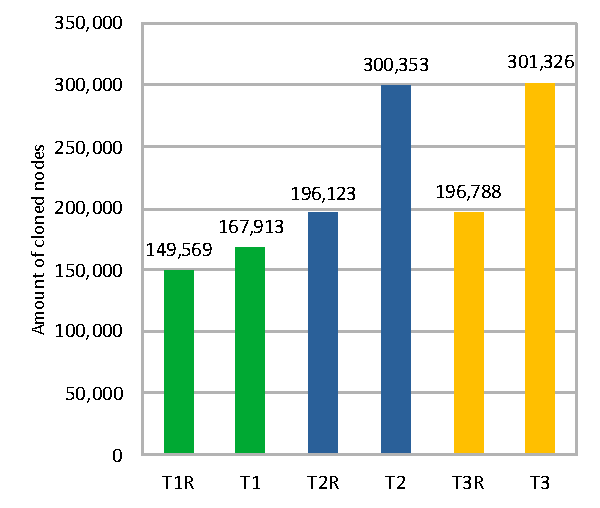
\includegraphics[width=\textwidth]{img/TypeResults}
    \caption{Number of cloned nodes.}
\label{fig:typeres}
  \end{minipage}
  \hfill
  \begin{minipage}[b]{0.45\textwidth}
    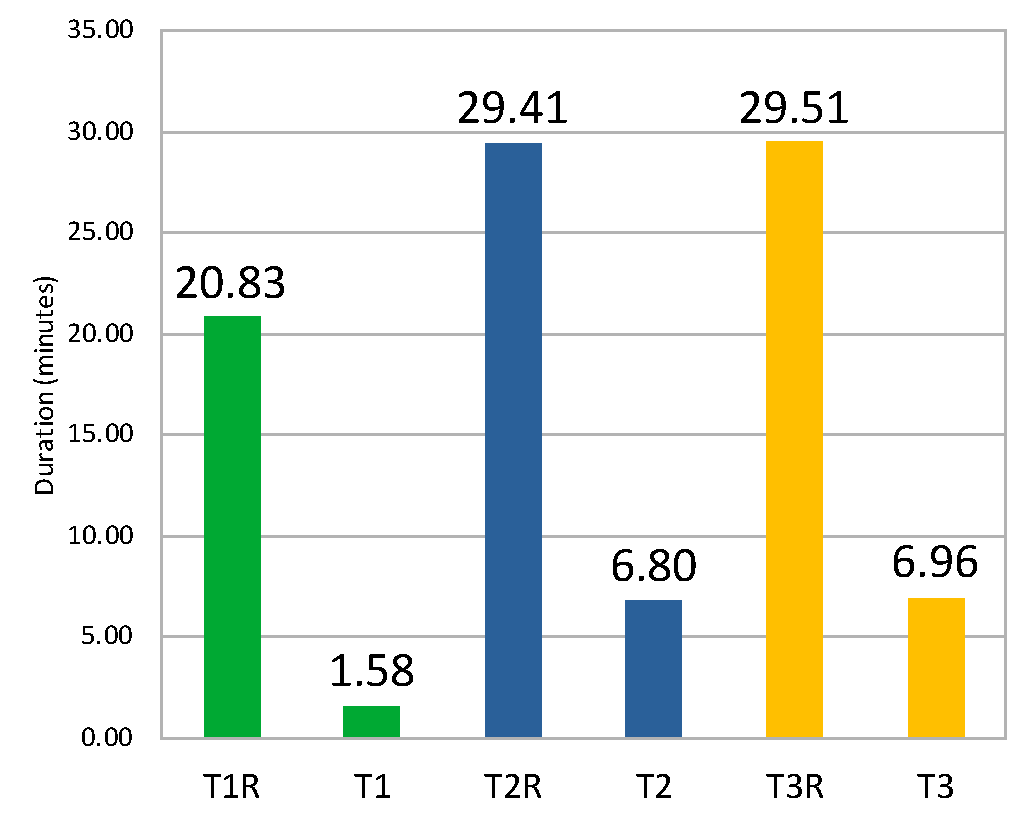
\includegraphics[width=\textwidth]{img/DurationChart}
    \caption{Clone type performance.}
  \label{fig:performance}
  \end{minipage}
\end{figure}

In Figure \ref{fig:typeres} we see that the difference between T1R and T1 is relatively small (11\% more cloned nodes found for T1). The difference between T2R and T2 is bigger (35\% more cloned nodes for T2). The number of cloned nodes of T3R and T3 are only a little bit higher than T2R and T2.

\subsection{Performance}
To map the viability of refactoring-oriented clone types for large scale clone detection, we measured the duration of finding clones by the different clone types. Figure~\ref{fig:performance} shows the duration of detecting all clones in the corpus using CloneRefactor for different clone types. This figure shows the average duration of running CloneRefactor 10 times for a certain clone type. We ran these performance tests on the compute nodes of the DAS4 supercomputer \cite{bal2016medium}, which allow for higher accuracy performance measurements as they do have limited background processes affecting the results.

\subsection{Type 2R Variability Threshold}
To determine the influence of the type 2R variability threshold on the amount of found nodes, we ran CloneRefactor for all variability percentages (0\% meaning no variance in expressions, 100\% meaning any variance in expressions). Figure \ref{fig:t2rgraph} shows the results.

\begin{figure}[H]
  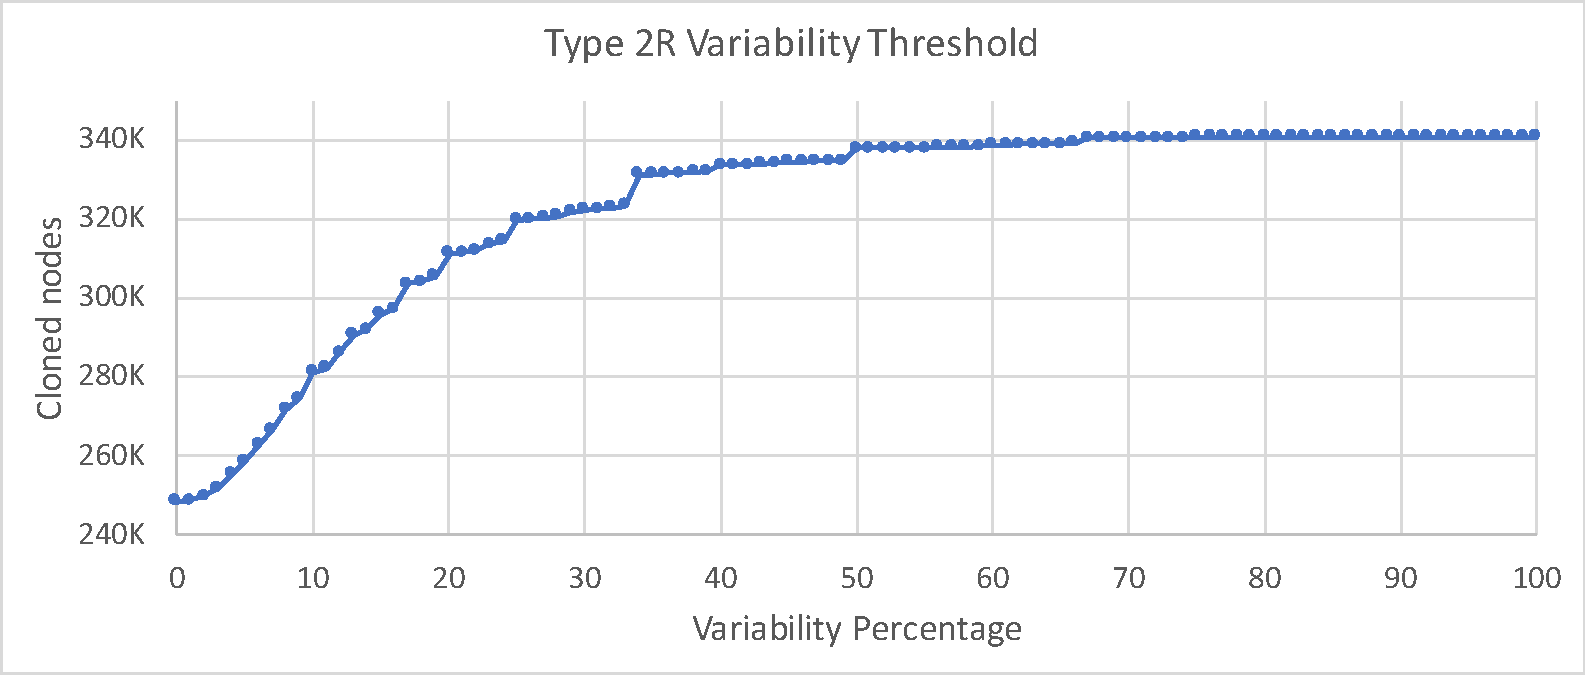
\includegraphics[width=1\textwidth]{img/T2R}
  \caption{Cloned nodes found for different Type 2R thresholds.}
  \label{fig:t2rgraph}
\end{figure}

In this graph, we see that the amount of clones increases as the amount of variability allowed increases. The graph is logarithmic: as the variability increases, the increase in nodes decreases.

\subsection{Type 3R Gap Size Thresholds}
To determine the influence of the type 3R gap size threshold on the amount of found nodes, we ran CloneRefactor for all gap size percentages between 0\% and 200\%. Figure \ref{fig:t3rgraph} shows the results.

\begin{figure}[H]
  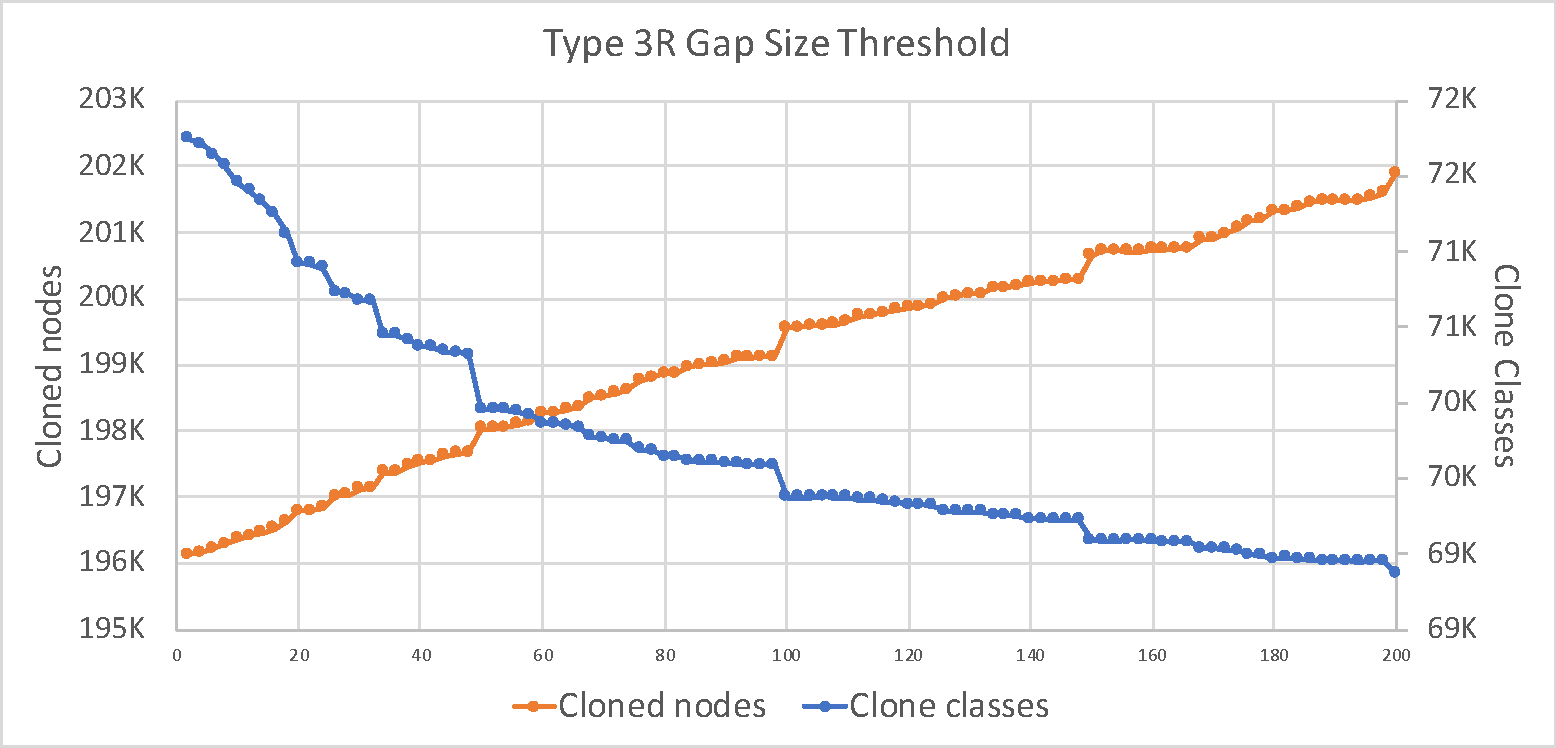
\includegraphics[width=1\textwidth]{img/T3R}
  \caption{Cloned nodes and clone classes found for different Type 3R thresholds.}
  \label{fig:t3rgraph}
\end{figure}

In this graph, we see a decrease in clone classes and an increase in cloned nodes when we increase the type 3R gap size threshold. We measure this threshold for a gap size of 0-200\%. In the graph, we see that both lines are rather linearly with minor jumps at certain thresholds. The jumps are at 33\%, 50\%, 100\%, 150\% and 200\%. The jump at 50\% is the largest. This makes sense regarding the nature of the threshold. At 50\%, all clone instances of 2 nodes with a gap of one node will merge into type 3R clones.

\section{Clone context}
% How many clones are there in certain contexts? Experiments for relation, location, and context.
To determine the refactoring method(s) that can be used to refactor most clones, we perform statistical analysis on the context of clones (see Section~\ref{chap:contextsetup}).

\subsection{Relation} \label{sec:relationresults}
Table~\ref{tab:relation} displays the number of clone classes found for the entire corpus for different relations (see Section~\ref{sec:setuprelation}).
% Sander: is dat plaatje met overzicht van relaties van clone classen weg of ergens anders? hij is hier ook wel handig

\begin{table}[H]
\centering
\begin{tabular}{@{}llrrrr@{}}
\toprule
\textit{\textbf{Category}} & \textit{\textbf{Relation}} & \textit{\textbf{Clone Classes}} & \textit{\textbf{\%}} & \textit{\textbf{Total}} & \textit{\textbf{\%}} \\ \midrule
\multirow{2}{*}{Common Class} & Same Class & 22,893 & 26.8\% & \multirow{2}{*}{31,848} & \multirow{2}{*}{37.2\%} \\ \cmidrule(lr){2-4}
 & Same Method & 8,955 & 10.5\% & & \\ \midrule
\multirow{5}{*}{Common Hierarchy} & Sibling & 15,588 & 18.2\% & \multirow{5}{*}{20,342}& \multirow{5}{*}{23.8\%} \\ \cmidrule(lr){2-4}
 & Superclass & 2,616 & 3.1\% & & \\ \cmidrule(lr){2-4}
 & First Cousin & 1,219 & 1.4\% & & \\ \cmidrule(lr){2-4}
 & Common Hierarchy & 720 & 0.8\% & & \\ \cmidrule(lr){2-4}
 & Ancestor & 199 & 0.2\% & & \\ \midrule
\multirow{4}{*}{Unrelated} & No Direct Superclass & 10,677 & 12.5\% & \multirow{4}{*}{20,314}& \multirow{4}{*}{23.7\%} \\ \cmidrule(lr){2-4}
 & External Superclass & 4,525 & 5.3\% & & \\ \cmidrule(lr){2-4}
 & External Ancestor & 3,347 & 3.9\% & & \\ \cmidrule(lr){2-4}
 & No Indirect Superclass & 1,765 & 2.1\% & & \\ \midrule
\multirow{2}{*}{Common Interface} & Same Direct Interface & 7,522 & 8.8\% & \multirow{2}{*}{13,074} & \multirow{2}{*}{15.3\%} \\ \cmidrule(lr){2-4}
 & Same Indirect Interface & 5,552 & 6.5\% & & \\ \bottomrule
\end{tabular}
\caption{Number of clone classes per clone relation.}
\label{tab:relation}
\end{table}

Our results show that most clones (37\%) are in a common class. 24\% of clones are in a common hierarchy. Another 24\% of clones are unrelated. 15\% of clones are in an interface.

\subsection{Location}
Table~\ref{tab:contents} displays the number of clone classes found for the entire corpus for different locations (see Section~\ref{sec:setuplocation}).
\begin{table}[H]
\centering
\begin{tabular}{@{}lrr@{}}
\toprule
\textit{\textbf{Category}} & \textit{\textbf{Clone instances}} & \textit{\textbf{\%}} \\ \midrule
Method Level & 232,545 & 78.43\% \\
Class Level & 50,402 & 17.00\% \\
Constructor Level & 10,039 & 3.39\% \\
Interface Level & 2,693 & 0.91\% \\
Enum Level & 788 & 0.27\% \\
\end{tabular}
\caption{Amount of clone instances with a per location category.}
\label{tab:location}
\end{table}

We can see from these results that most clones are found at method level.

\subsection{Contents}
Table~\ref{tab:contents} displays the number of clone classes found for the entire corpus for different contents (see Section~\ref{sec:setupcontents}).

\begin{table}[H]
\centering
\begin{tabular}{@{}llrrrr@{}}
\toprule
\textit{\textbf{Category}} & \textit{\textbf{Contents}} & \textit{\textbf{Clone instances}} & \textit{\textbf{Total}} \\ \midrule
\multirow{2}{*}{Partial} & Partial Method & 219,540 & 74.05\% & \multirow{2}{*}{229,521}& \multirow{2}{*}{77.42\%} \\ \cmidrule(lr){2-4}
 & Partial Constructor & 9,981 & 3.37\% & & \\ \midrule
\multirow{5}{*}{Full} & Full Method & 12,990 & 4.38\% & \multirow{5}{*}{13,173}& \multirow{5}{*}{4,44\%} \\ \cmidrule(lr){2-4}
 & Full Interface & 64 & 0.02\% & & \\ \cmidrule(lr){2-4}
 & Full Constructor & 58 & 0.02\% & & \\ \cmidrule(lr){2-4}
 & Full Class & 37 & 0.01\% & & \\ \cmidrule(lr){2-4}
 & Full Enum & 24 & 0.01\% & & \\ \midrule
\multirow{3}{*}{Other} & Several Methods & 22,749 & 7.67\% & \multirow{3}{*}{53,773} & \multirow{3}{*}{18.14\%} \\ \cmidrule(lr){2-4}
 & Only Fields & 17,700 & 5.97\% & & \\ \cmidrule(lr){2-4}
 & Other & 13,324 & 4.49\% & & \\ \bottomrule
\end{tabular}
\caption{Number of clone instances for clone contents categories}
\label{tab:contents}
\end{table}

From these results, we see that 74\% of clones span part of a method body (77\% if we include constructors). 8\% of clones span several methods. 6\% of clones span only global variables. Only 4\% of clones span a full declaration (method, class, constructor, etc.).

\section{Refactorability}
%To what extent can found clones be refactored through method extraction, without requiring additional transformations.
Table~\ref{tab:refactorability} shows to what extent clone classes can be refactored by using the ``Extract Method'' refactoring technique. The second column shows our measurements for the complete systems (just like the former experiments).
\begin{table}[H]
\centering
\begin{tabular}{@{}lrr@{}}
\toprule
\textit{\textbf{Category}} & \textit{\textbf{All}} & \textit{\textbf{\% (All)}} \\ \midrule
Can Be Extracted & 24,157 & 28.2\%  \\
Is Not A Partial Method & 21,625 & 25.3\% \\
Top-level AST-Node is not a Statement & 19,887 & 23.2\% \\
Spans Part of a Block & 12,964 & 15.2\%  \\
Multiple Return Values & 5,622 & 6.6\%  \\
Complex Control Flow & 1,106 & 1.3\% \\
Overlap In Clone Class & 147 & 0.2\% \\
Not In Class Or Interface & 70 & 0.1\% \\
\bottomrule
\end{tabular}
\caption{Number of clones that can be extracted using the ``Extract Method'' refactoring technique}
\label{tab:refactorability}
\end{table}

\section{Thresholds} \label{sec:refactoringexperiments}
%I think the ultimate goal with this thesis is to do experiments with different clone thresholds. Which thresholds give clones that we should refactor? For this, we will measure the maintainability of the refactored source code over different thresholds. These thresholds range from minimum clone size, variability, and gap size.
In our corpus, CloneRefactor has refactored 12,710 clone classes and measured the change in indicated metrics (see Section~\ref{sec:metrics}). Using the presented formulas (see Section~\ref{sec:metricformula}) we determine how the characteristics of the extracted method (see Section~\ref{sec:characteristics}) influence the maintainability of the resulting codebase after refactoring. In this section, we explore the data received by comparing the before- and after snapshots of the system for each separate refactoring. Using this data, we find supporting evidence regarding which thresholds are most likely to find clones that should be refactored to improve maintainability.

We use the following keywords as headers of the columns of our tables:
\begin{itemize}
  \item \textbf{Complexity}: The average delta complexity for all refactored clone classes in the specified category.
  \item \textbf{Parameters}: The average delta number of parameters for all refactored clone classes in the specified category.
  \item \textbf{Volume}: The average delta number of tokens for all refactored clone classes in the specified category.
  \item \textbf{Duplication}: The average delta number of duplicate tokens for all refactored clone classes in the specified category.
  \item \textbf{\#}: The number of times the specified category is refactored (and thus the number of data points we have for this category).
  \item \textbf{Score}: The average delta maintainability score (see Section~\ref{sec:metricformula} for the formula by which this score is calculated) for all refactored clone classes in the specified category.
\end{itemize}
In this context, the \textit{delta} denotes the change in this metric between the before- and after-refactoring snapshot of the system, for each separate clone class that was refactored.

\subsection{Clone Token Volume}
Figure \ref{fig:maintainabilityscore} shows the obtained results when plotting the clone volume against the maintainability increase/decrease. We define the \textit{token volume} as the combined number of tokens in all clone instances in a refactored clone class. The maintainability score, as shown in Figure \ref{fig:maintainabilityscore}, is the average delta maintainability score of all clone classes with the specified token volume that are refactored. For larger token volumes we have fewer refactorings that refactor such clones, because of which we represent the x-axis as a logarithmic scale. The trendline intersects the ``zero'' line (maintainability does not increase nor decrease) at a token volume of 63.

\begin{figure}[H]
  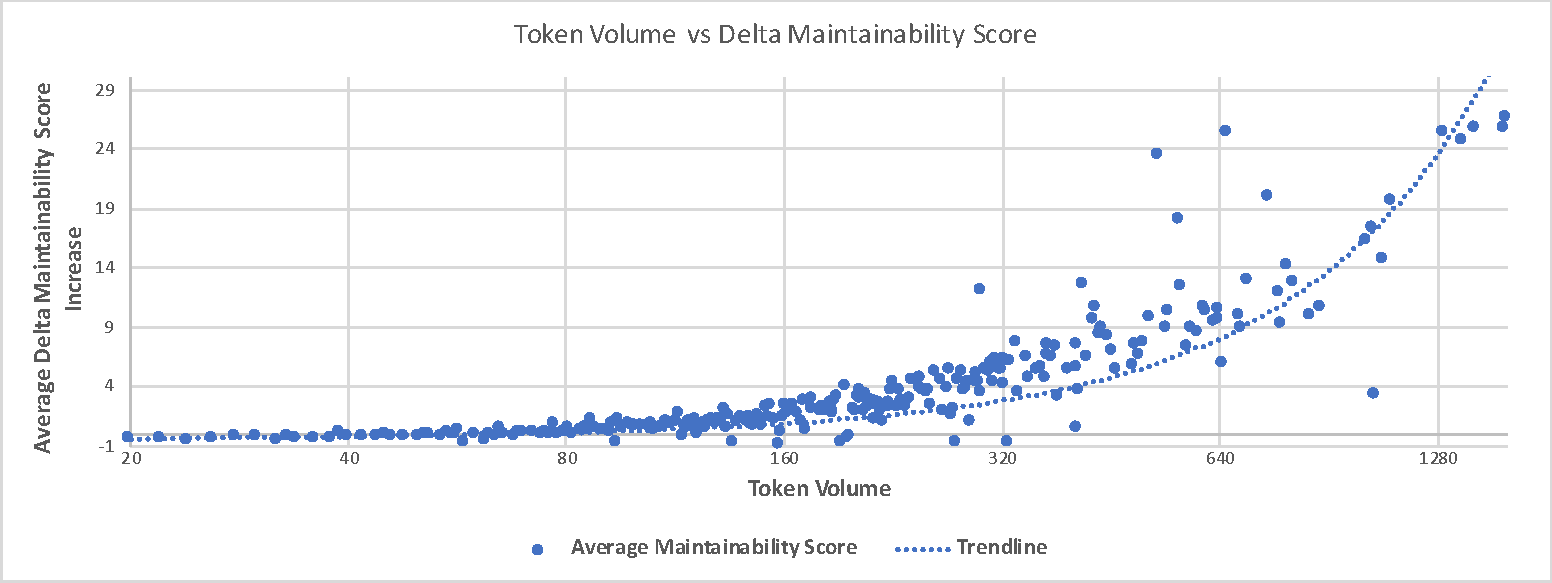
\includegraphics[width=1\textwidth]{img/maintainabilityscore}
  \caption{The effect of token volume on the delta maintainability score of the refactored clones}
  \label{fig:maintainabilityscore}
\end{figure}

The token volume of the clone is equal to the decrease of duplicated tokens, which is part of the maintainability score. Because of that, what we see in Figure~\ref{fig:maintainabilityscore} could largely be caused by this metric. To determine the effect of clone token volume on each metric, we also plot graphs in which each metric is considered singularly. In Figure~\ref{fig:volume} the average delta volume is shown when clones with the specified token volume are refactored. The trendline intersects the ``zero'' line (average delta volume does not increase nor decrease) at 60 tokens. A higher average delta volume implies lower maintainability.

\begin{figure}[H]
  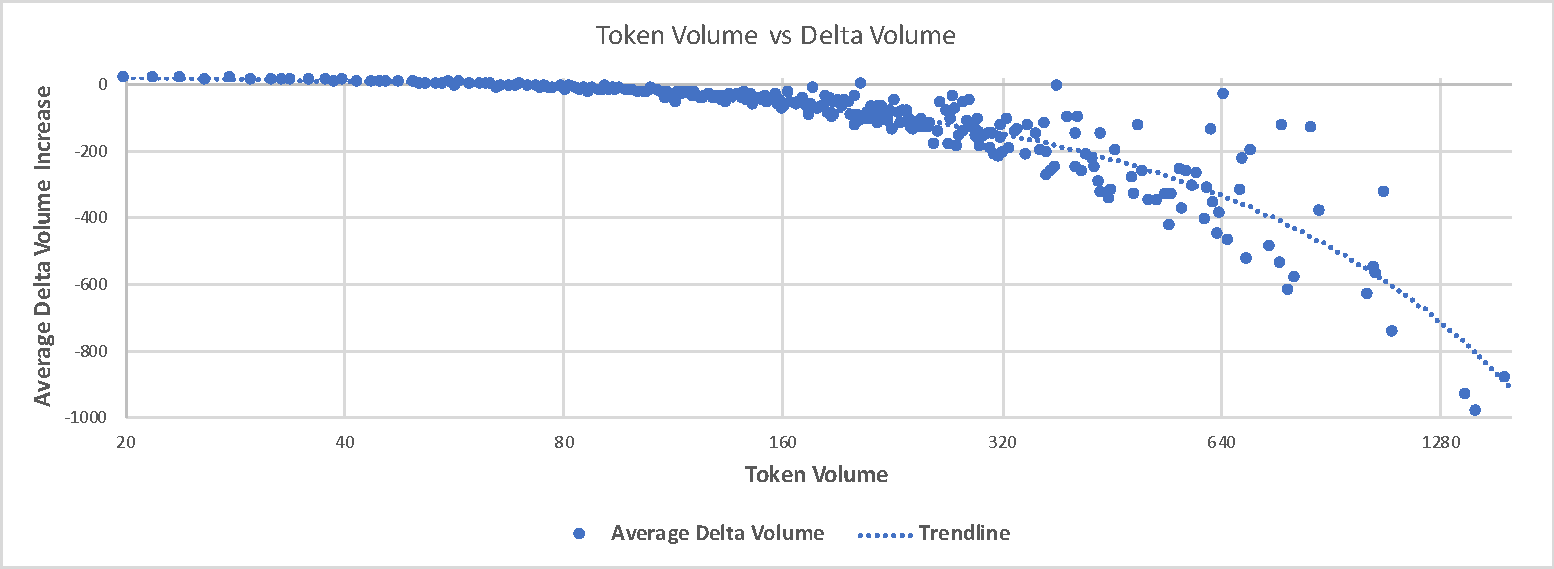
\includegraphics[width=1\textwidth]{img/volume}
  \caption{The effect of token volume on the delta volume of the refactored clones}
  \label{fig:volume}
\end{figure}

In Figure~\ref{fig:numberofparameters} we show the average delta number of parameters when clones with the specified token volume are refactored. This metric can only increase by the refactoring because CloneRefactor only applies ``Extract Method'' refactorings that create a method with a certain number of parameters (according to the data needed by the extracted method).

\begin{figure}[H]
  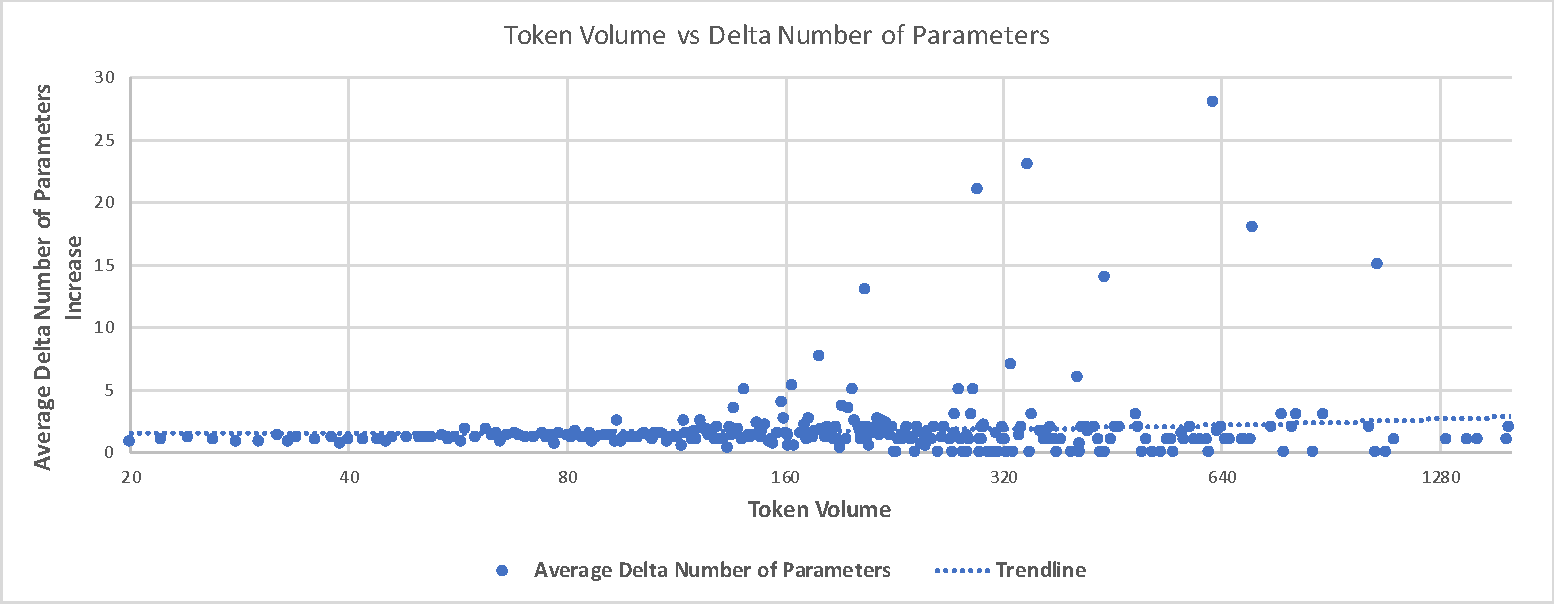
\includegraphics[width=1\textwidth]{img/numberofparameters}
  \caption{The effect of token volume on the number of parameters of the refactored clones}
  \label{fig:numberofparameters}
\end{figure}

In Figure~\ref{fig:complexity} we show the average delta complexity when clones with the specified token volume are refactored. We did not add a trendline, as there does not seem to be a clear trend. The maximum delta complexity is one because the extracted method itself has a complexity of one. For each branching point in the cloned fragment, the complexity of the system will decrease when such a clone is refactored.

\begin{figure}[H]
  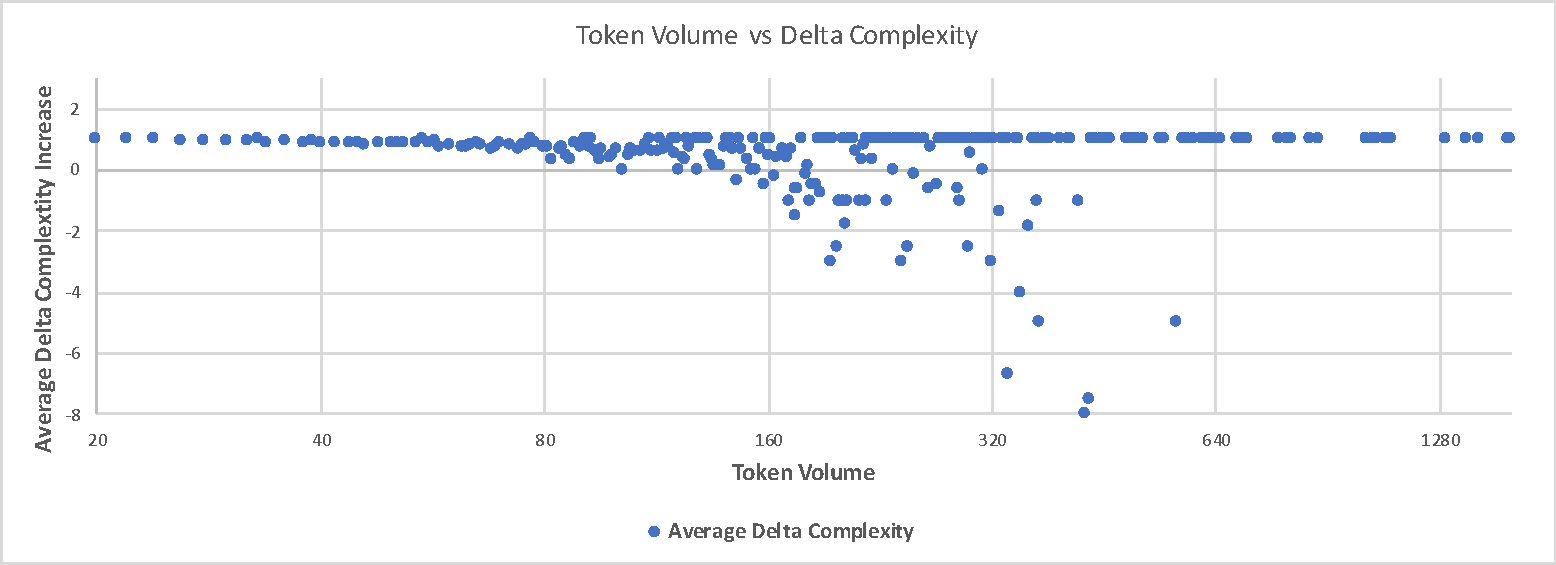
\includegraphics[width=1\textwidth]{img/complexity}
  \caption{The effect of token volume on the complexity of the refactored clones}
  \label{fig:complexity}
\end{figure}

\subsection{Relation}
Table~\ref{tab:relationref} shows our data regarding how different relations influence maintainability. We mark rows based on less than 100 refactorings red, as their result might not have statistical significance. The \textbf{Relation} column refers to the relations introduced in Section~\ref{sec:setuprelation}. Relations are mutually exclusive so all percentages add up to 100\%.

\begin{table}[H]
\centering
\resizebox{\textwidth}{!}{%
\begin{tabular}{@{}lrrrrrr@{}}
\toprule
\textit{\textbf{Relation}} & \textit{\textbf{Duplication}} & \textit{\textbf{Complexity}} & \textit{\textbf{Parameters}} & \textit{\textbf{Volume}} & \textit{\textbf{\#}} & \textit{\textbf{Score}} \\ \midrule
\textbf{Common Hierarchy} & \textbf{-66.33} & \textbf{0.73} & \textbf{1.20} & \textbf{-8.85} & \textbf{2,202} & \textbf{0.23} \\ \midrule
\hspace{10pt} Superclass & -64.48 & 0.79 & 0.94 & -7.22 & 229 & 0.42 \\
\hspace{10pt} Sibling & -70.07 & 0.69 & 1.28 & -10.97 & 1,722 & 0.23 \\
\rowcolor[HTML]{FFCCC9}
\hspace{10pt} Same Hierarchy & -44.18 & 0.95 & 0.89 & 1.54 & 87 & 0.10 \\
\hspace{10pt} First Cousin & -42.69 & 0.89 & 0.93 & 4.86 & 144 & 0.02 \\
\rowcolor[HTML]{FFCCC9}
\hspace{10pt} Ancestor & -32.75 & 1.00 & 0.75 & 11.00 & 20 & -0.03 \\ \midrule
\textbf{Common Interface} & \textbf{-47.06} & \textbf{0.83} & \textbf{1.04} & \textbf{4.50} & \textbf{1,044} & \textbf{-0.02} \\ \midrule
\hspace{10pt} Same Indirect Interface & -37.08 & 0.93 & 0.82 & 9.96 & 487 & -0.01 \\
\hspace{10pt} Same Direct Interface & -55.79 & 0.75 & 1.24 & -0.28 & 557 & -0.02 \\ \midrule
\textbf{Common Class} & \textbf{-52.42} & \textbf{0.87} & \textbf{1.13} & \textbf{1.47} & \textbf{7,239} & \textbf{-0.02} \\ \midrule
\hspace{10pt} Same Class & -51.85 & 0.86 & 1.03 & 3.36 & 4,874 & 0.04 \\
\hspace{10pt} Same Method & -53.60 & 0.90 & 1.32 & -2.44 & 2,365 & -0.15 \\ \midrule
\textbf{Unrelated} & \textbf{-45.86} & \textbf{0.88} & \textbf{1.08} & \textbf{9.56} & \textbf{2,198} & \textbf{-0.15} \\ \midrule
\hspace{10pt} No Direct Superclass & -52.24 & 0.84 & 1.12 & 6.04 & 811 & -0.06 \\
\hspace{10pt} External Superclass & -47.09 & 0.87 & 1.13 & 8.77 & 697 & -0.17 \\
\hspace{10pt} External Ancestor & -35.73 & 0.93 & 0.95 & 14.58 & 586 & -0.21 \\
\hspace{10pt} No Indirect Superclass & -44.89 & 0.84 & 1.18 & 14.08 & 104 & -0.30 \\ \midrule
\textbf{Grand Total} & \textbf{-53.26} & \textbf{0.84} & \textbf{1.12} & \textbf{1.33} & \textbf{12,683} & \textbf{0.00} \\ \bottomrule
\end{tabular}%
}
\caption{Average metric values for refactorings of clone classes with the specified relations}
\label{tab:relationref}
\end{table}

The displayed relations are ordered by their scores. Overall, the scores do not deviate much (-0.15 to 0.23), indicating that the relation between clones has a minor impact on maintainability. Overall, we see that common hierarchy clones have the highest maintainability, whereas unrelated clones have the lowest maintainability.

\subsection{Return Category}
Table~\ref{tab:return} shows how the return value of the extracted method influences the maintainability of the resulting system. The \textbf{Return Category} column refers to the categories introduced in Section~\ref{sec:refreturn}.

\begin{table}[H]
\centering
%\resizebox{\textwidth}{!}{%
\begin{tabular}{@{}lrrrrrr@{}}
\toprule
\textit{\textbf{Return Category}} & \textit{\textbf{Complexity}} & \textit{\textbf{Parameters}} & \textit{\textbf{Size}} & \textit{\textbf{Duplication}} & \textit{\textbf{\#}} & \textit{\textbf{Score}} \\ \midrule
Return & 0.85 & 1.02 & -3.84 & -55.00 & 1,571 & 0.19 \\
Declare & 0.94 & 0.74 & 11.11 & -49.19 & 5,177 & 0.15 \\
\rowcolor[HTML]{FFCCC9}
Assign & 0.79 & 1.07 & 0.43 & -56.29 & 14 & 0.12 \\
Void & 0.76 & 1.49 & -5.85 & -56.35 & 5,921 & -0.18 \\ \midrule
\textbf{Grand Total} & \textbf{0.84} & \textbf{1.12} & \textbf{1.33} & \textbf{-53.26} & \textbf{12,683} & \textbf{0.00} \\ \bottomrule
\end{tabular}%
%}
\caption{Average metric values for refactorings of clone classes with the specified return category}
\label{tab:return}
\end{table}

The displayed return categories are ordered by their scores. Overall, the scores do not deviate much (-0.18 to 0.19), indicating that the return category has a minor impact on maintainability. When the result of the call to the extracted method is directly returned, the maintainability score is the highest. When no value is returned, the maintainability score is the lowest. The main reason that no return value ends up lowest, is that it is linked to a higher number of parameters required for the extracted method.

\subsection{Parameters}
Fig.~\ref{fig:arguments} shows how an increase in parameters lowers the maintainability of the refactored code. On the primary x-axis, the maintainability is displayed. The secondary x-axis shows the number of refactorings. The y-axis shows the number of parameters. The table containing all underlying data and separate metrics is displayed in Appendix~\ref{sec:parameterstable}.

\begin{figure}[H]
  \centering
  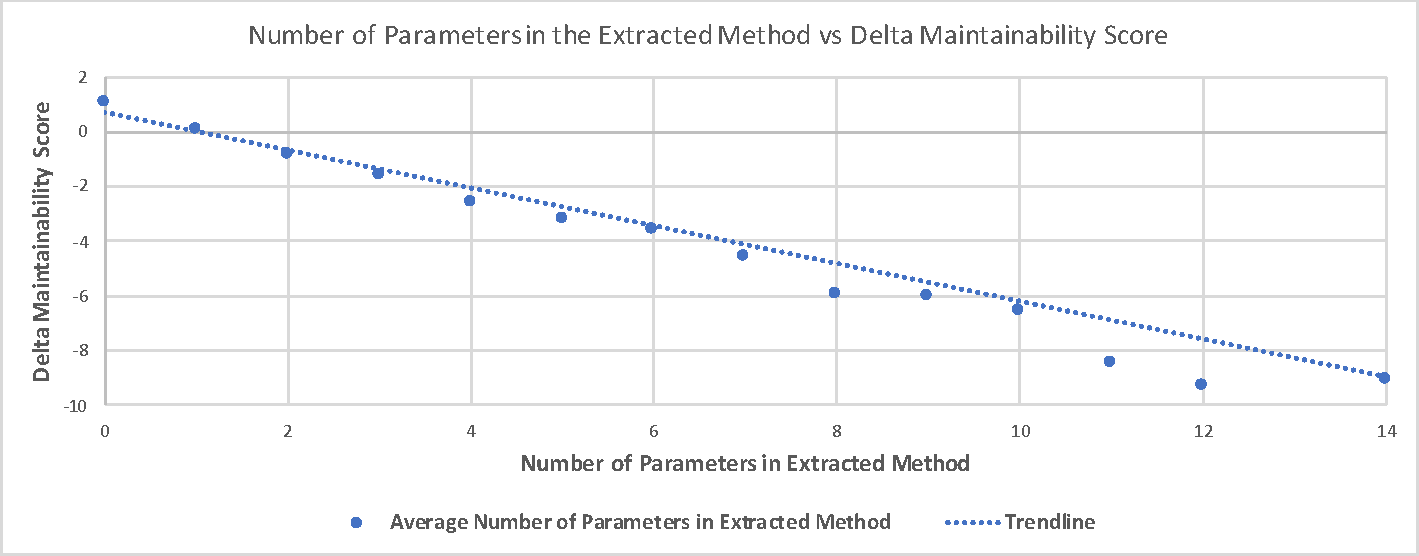
\includegraphics[width=0.8\columnwidth]{img/arguments}
  \caption{Influence of number of method parameters on system maintainability.}
  \label{fig:arguments}
\end{figure}
